\documentclass[aspectratio=169,11pt]{beamer}

\usetheme{Madrid}
\usecolortheme{default}
\usefonttheme{professionalfonts}
\setbeamertemplate{navigation symbols}{}
\setbeamertemplate{footline}[frame number]

\usepackage{amsmath, amssymb, booktabs, graphicx}
\graphicspath{{../../assets/figures/}{assets/figures/}}

\title{Dynamic Labor Demand and Adjustment Costs}
\subtitle{Labor II --- Week 2}
\author{Teaching deck draft}
\date{}

\begin{document}

\begin{frame}
  \titlepage
\end{frame}

\begin{frame}{Central question}
\begin{itemize}
    \item Why do firms adjust employment slowly after shocks?
    \item Which cost structures generate smooth responses versus inaction and lumpiness?
    \item Why do policy effects depend on the adjustment path rather than only the new target?
\end{itemize}
\end{frame}

\begin{frame}{Week 1 to Week 2 bridge}
\begin{itemize}
    \item Week 1 derived the firm's static labor-demand target.
    \item Week 2 asks why actual employment does not jump immediately to that target.
    \item Week 3 will stay inside the firm and ask how personnel design changes internal adjustment.
\end{itemize}
\end{frame}

\begin{frame}{Target versus actual employment}
\[
L_t^{\ast} = L^{\ast}(w_t, p_t, K_t, A_t, q_t)
\]

\begin{itemize}
    \item The target is the Week 1 destination.
    \item The Week 2 object is the gap between actual employment and that target.
    \item The horizon matters: hours, headcount, hiring, and firing need not move together.
\end{itemize}
\end{frame}

\begin{frame}{Target versus actual after a shock}
\begin{center}
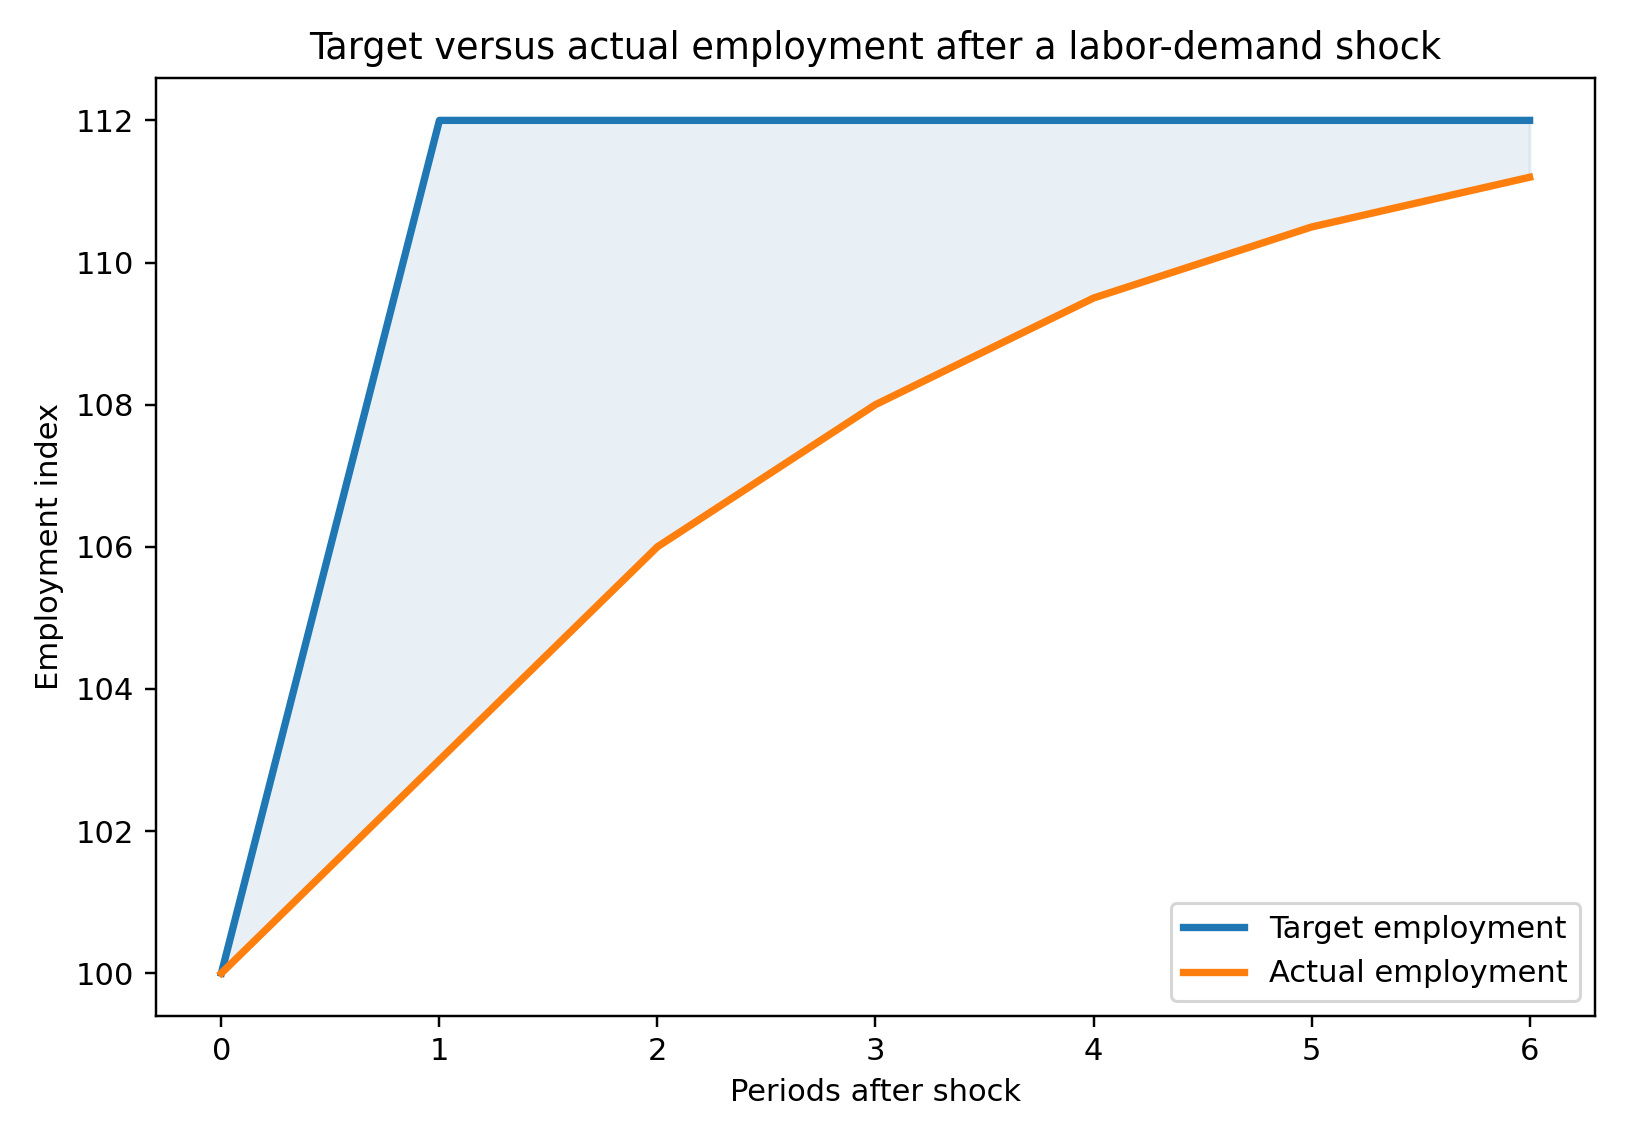
\includegraphics[height=0.68\textheight]{02-target-vs-actual-employment.png}
\end{center}
\end{frame}

\begin{frame}{Dynamic objective with adjustment costs}
\[
V(L_{t-1}, s_t) =
\max_{L_t}
\left\{
\pi(L_t, s_t) - C(L_t-L_{t-1})
\;+\;
\beta E_t[V(L_t, s_{t+1})]
\right\}
\]

\begin{itemize}
    \item Yesterday's workforce is a state variable.
    \item Adjustment costs make current choices affect future payoffs.
    \item The cost function \(C(\cdot)\) is the central Week 2 object.
\end{itemize}
\end{frame}

\begin{frame}{Convex costs and partial adjustment}
\[
L_t - L_{t-1}
=
\lambda(L_t^{\ast} - L_{t-1}),
\qquad 0 < \lambda \le 1
\]

\begin{itemize}
    \item Convex costs imply frequent but modest adjustments.
    \item \(\lambda\) is a reduced-form speed-of-adjustment object.
    \item Short-run incidence can differ sharply from long-run incidence.
\end{itemize}
\end{frame}

\begin{frame}{Convex versus nonconvex adjustment}
\begin{center}
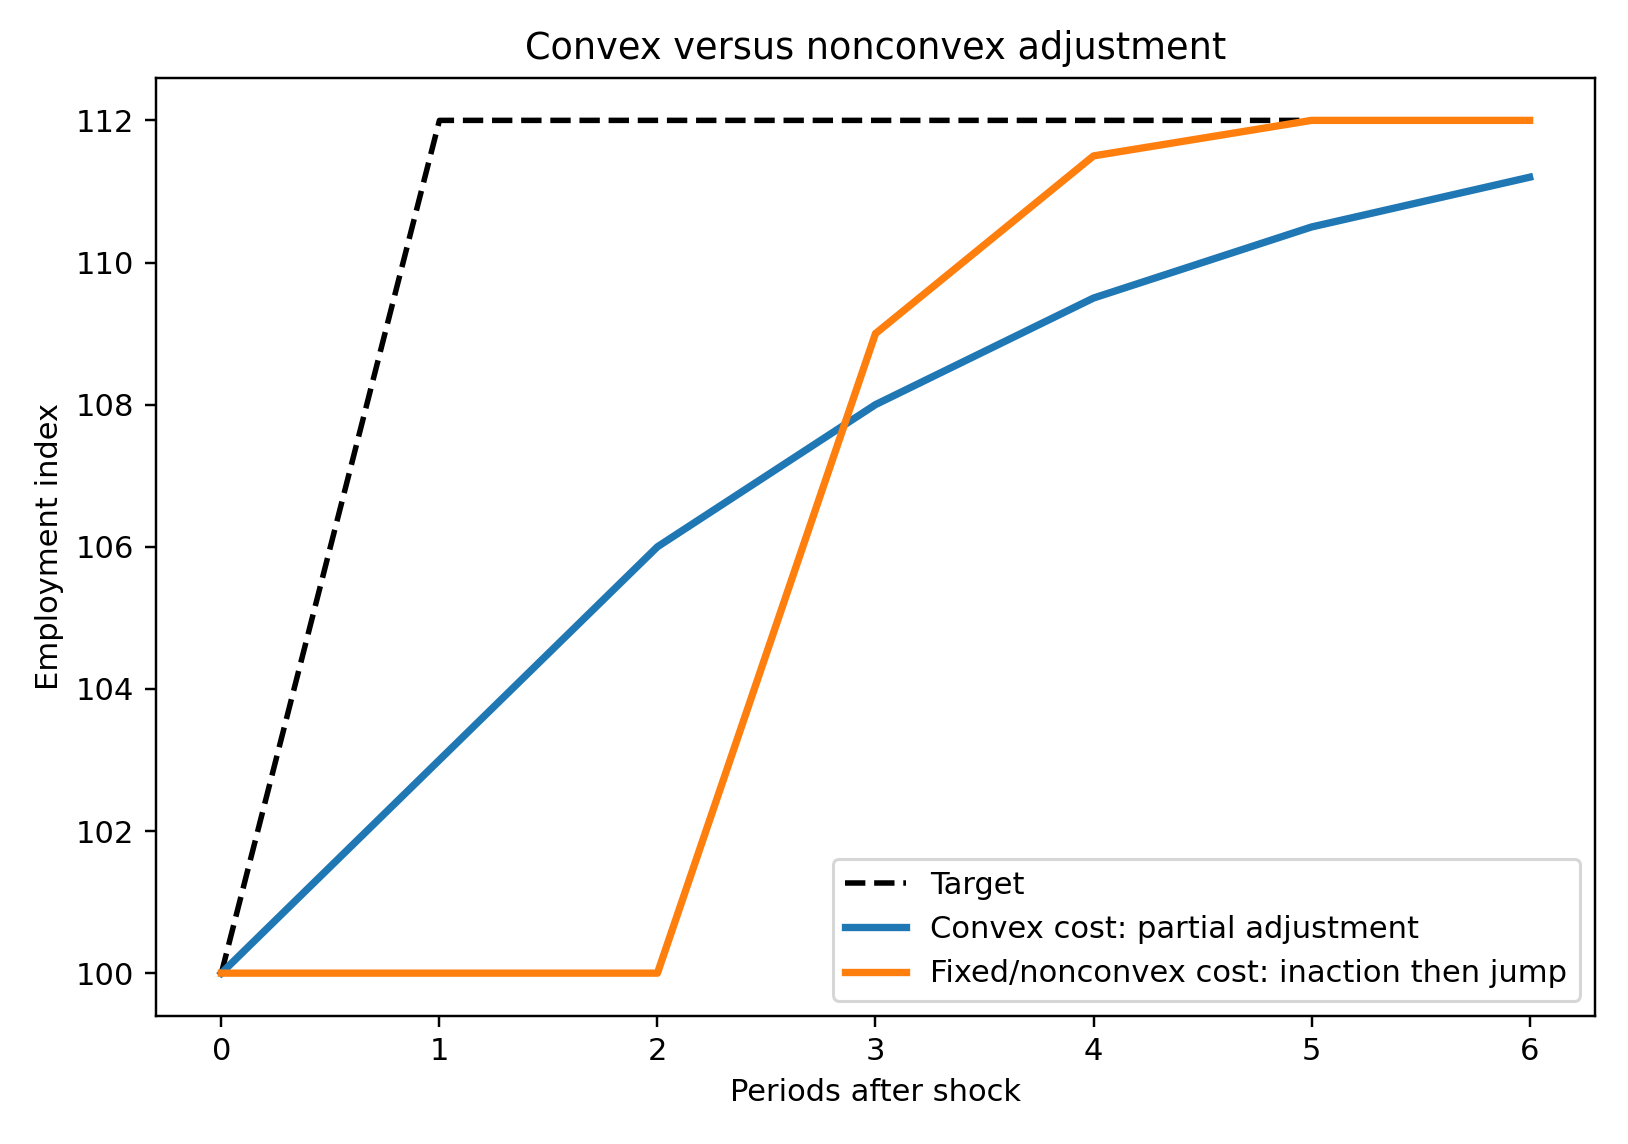
\includegraphics[height=0.68\textheight]{02-convex-vs-nonconvex-adjustment.png}
\end{center}
\end{frame}

\begin{frame}{Fixed or nonconvex costs}
\[
\text{adjust if }
\left|L_t^{\ast} - L_{t-1}\right| > \bar{\Delta}
\]

\begin{itemize}
    \item Small shocks generate inaction.
    \item Large shocks trigger lumpy adjustments.
    \item Plant-level zeros and spikes are hard to reconcile with a purely convex benchmark.
\end{itemize}
\end{frame}

\begin{frame}{Hours, headcount, hiring, and firing}
\begin{itemize}
    \item Hours often move before core headcount.
    \item Hiring margins are most visible after positive shocks.
    \item Separations and layoffs are most visible after negative shocks.
    \item Labor hoarding means weak headcount responses can still mask real labor-demand adjustment.
\end{itemize}
\end{frame}

\begin{frame}{Hours versus headcount}
\begin{center}
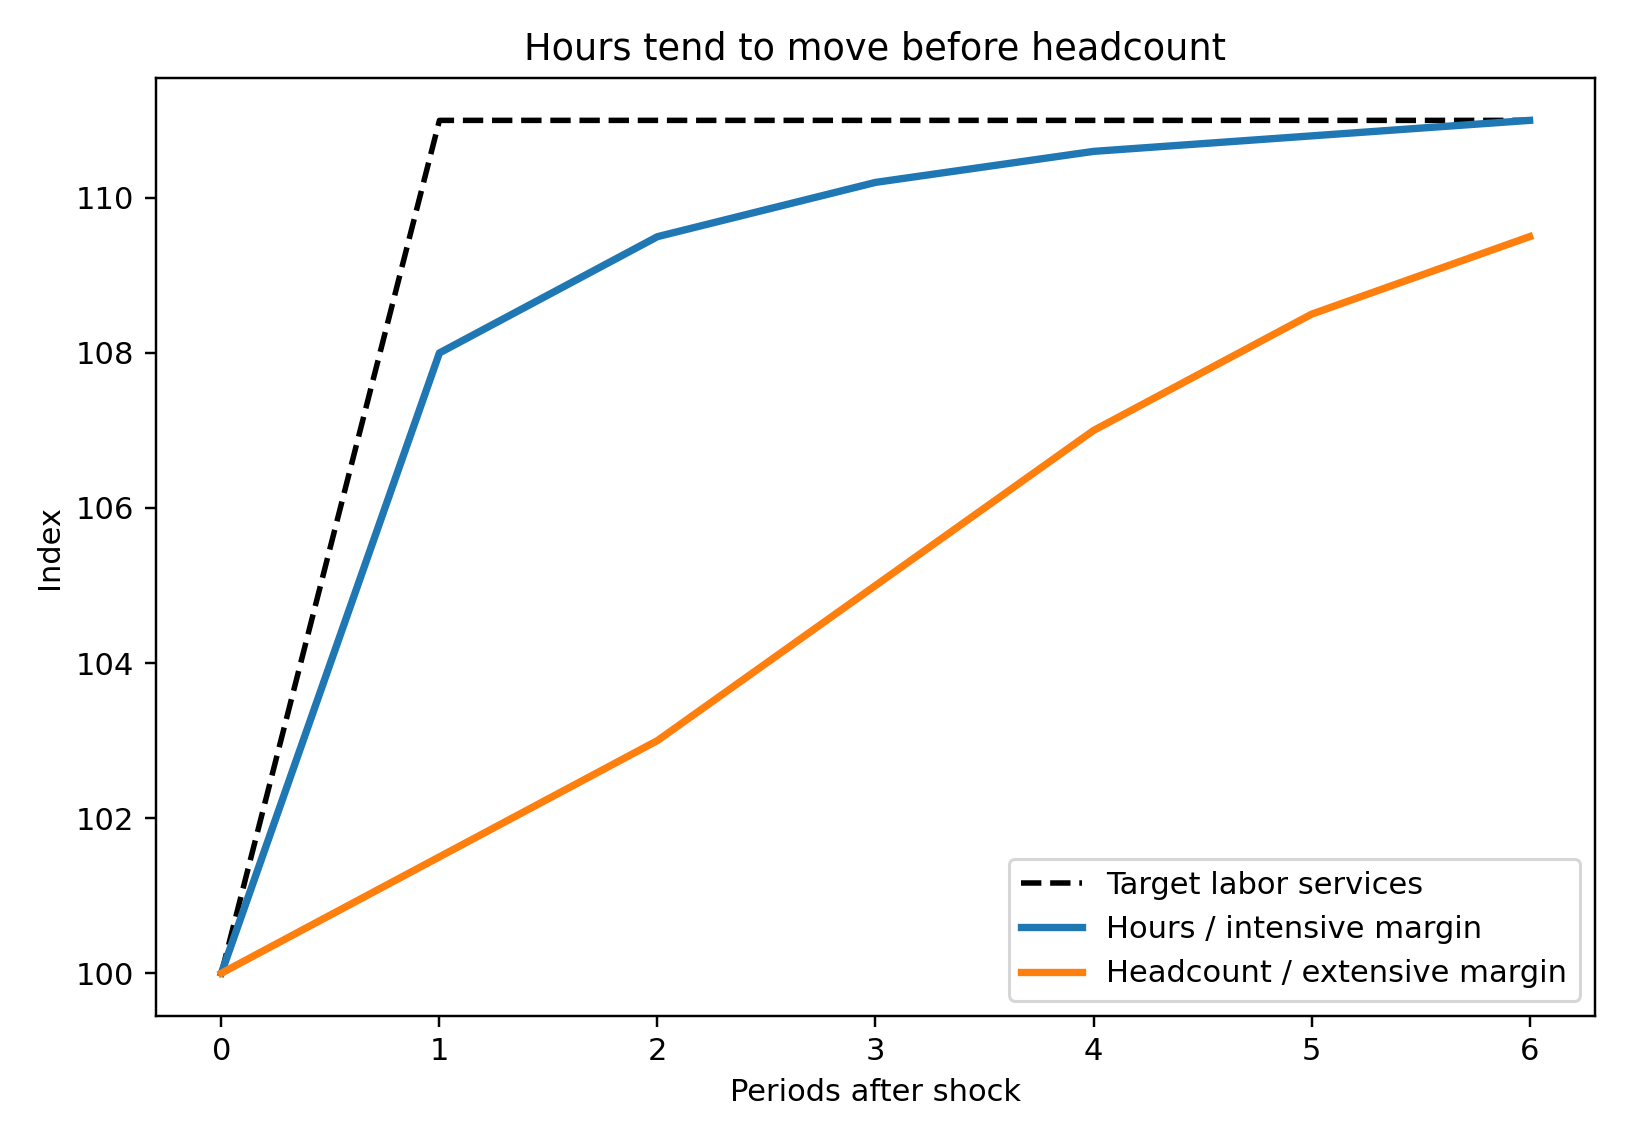
\includegraphics[height=0.68\textheight]{02-hours-vs-headcount-adjustment.png}
\end{center}
\end{frame}

\begin{frame}{Empirical designs and what they identify}
\small
\begin{tabular}{p{0.24\linewidth} p{0.22\linewidth} p{0.19\linewidth} p{0.23\linewidth}}
\toprule
Design & Variation & Margin & Dynamic object \\
\midrule
Plant panels & Within-firm dynamics & Employment, hours & Persistence, hazards, lumpiness \\
Policy timing & Labor-cost reform & Wages, employment, hours & Incidence over event time \\
Belief or uncertainty surveys & Firm expectations & Expected or realized employment & Delay and state dependence \\
Structural estimation & Model-implied states & Adjustment path & Deep cost parameters \\
\bottomrule
\end{tabular}
\end{frame}

\begin{frame}{Policy timing and incidence}
\[
\frac{\partial L_{t+h}}{\partial \tau_t},
\qquad h = 0,1,2,\ldots
\]

\begin{itemize}
    \item Dynamic policy effects are horizon-specific.
    \item Firms can adjust hours, vacancies, wages, prices, or headcount in sequence.
    \item Event studies and structural models answer related but different questions.
\end{itemize}
\end{frame}

\begin{frame}{Policy incidence over time}
\begin{center}
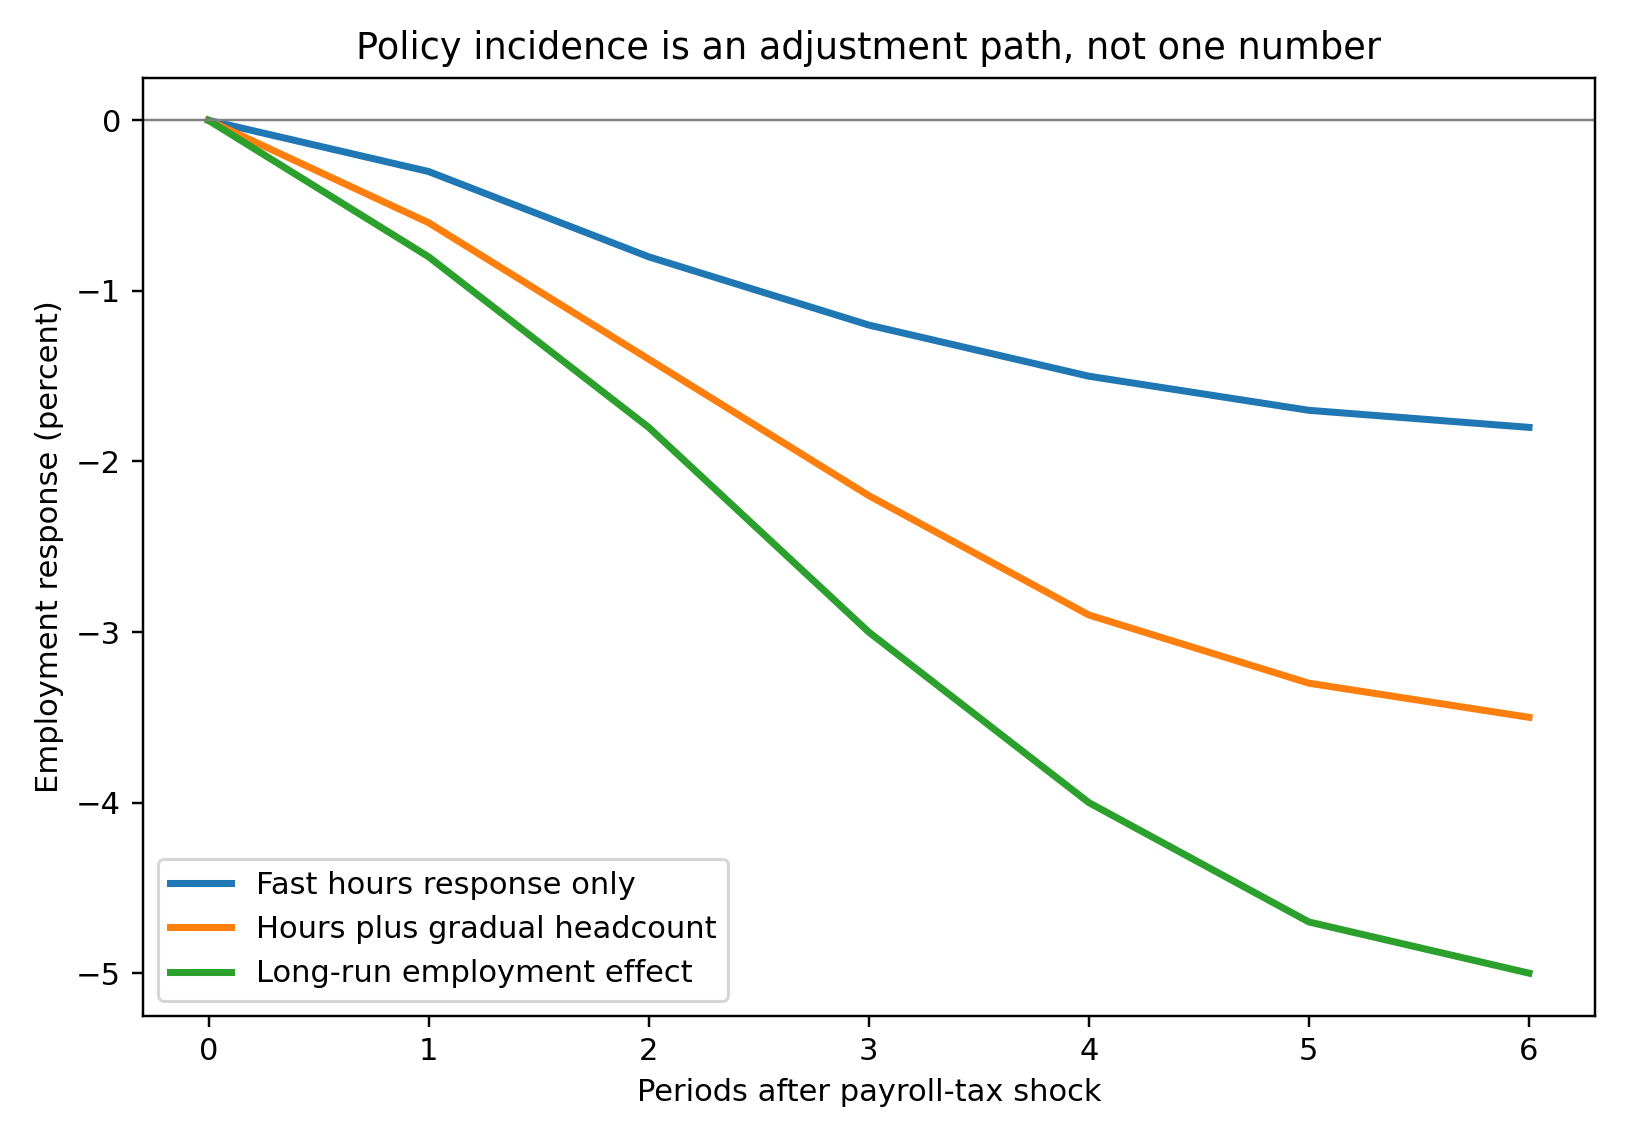
\includegraphics[height=0.68\textheight]{02-policy-incidence-over-time.png}
\end{center}
\end{frame}

\begin{frame}{Bridge to Week 3}
\begin{itemize}
    \item Week 2 explains why employment paths are slow and margin-specific.
    \item Week 3 asks how firms design incentives, promotions, and internal labor markets once those dynamic frictions exist.
    \item Dynamic adjustment is therefore the firm-side foundation for the personnel block.
\end{itemize}
\end{frame}

\begin{frame}{Takeaways}
\begin{itemize}
    \item Target employment and actual employment are different objects.
    \item Convex costs smooth responses; fixed or nonconvex costs create inaction and lumpiness.
    \item Hours, headcount, hiring, and firing reveal different adjustment margins.
    \item Policy incidence should be read over the adjustment path, not at one horizon only.
\end{itemize}
\end{frame}

\end{document}
